% !TeX root = ../../tfg.tex
% !TeX encoding = utf8
%
%***************************************************************
% Contenido del artículo 5: Generalización a multi-output 
%***************************************************************
\section{Generalización para \textit{multi-output neuronal networks}}

En las secciones anteriores se han provisto resultados para redes 
neuronales de salida real. Vamos a generalizar los resultados vistos
para ser capaces de aproximar funciones continuas o medibles 
de $\R^r$ a $\R^s$ con $r,s \in \N.$

Denotaremos como $\fCC$ al conjunto de funciones continuas definidas de $\R^r$ a $\R^s$ y al de funciones medibles de 
$\R^r$ a $\R^s$  como $\fMM.$ 
La distancia asociada a estos espacios se define como 
\begin{equation}
    \rho_{\mu}^s(f,g) 
    =
    \sum_{i=1}^s \dist(f_i, g_i).
\end{equation}

Con la siguiente definición buscamos abstraer el modelo de una red neuronal de una capa oculta y salida múltiple.
\begin{figure}[h]
    \centering
    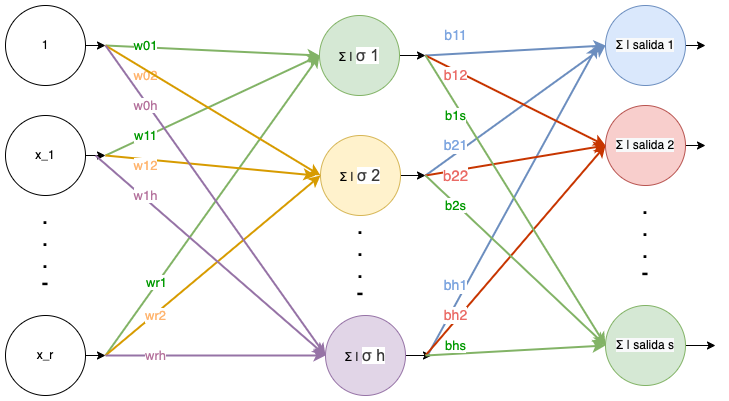
\includegraphics[width=.7\textwidth]{articulo_rrnn_aproximadores_universales/RedNeuronalAbstactaUnaCapaVariasSalidas.png}
    \caption{Ejemplo de red neuronal de una capa oculta con $h$ nodos, de dimensión de entrada $r$ y salida $s$.}
    \label{fig:red neuronal-r-h-s}
\end{figure}

Nótese que los vectores $(w_{0i},w_{1i}, \ldots, w_{ri})$ representan a la aplicación afín 
$A_i((x_1, x_2, \ldots x_r)) = w_{0i} + \sum_{j=1}^r w_{ji} x_j$
con $i \in \{1,\ldots, h\}$ . 

\begin{definicion}[Abstracción red neuronal una capa oculta múltiple salida] 
    Para cualquier función Borel medible $G$, definida de $\R$ a $\R$ y cualquier natural positivo
    $r \in \N$ se define a la clase de funciones $\pmc$ como 
    \begin{equation}
        \begin{split}
        \sum^{r,s}(G) = 
        \{ 
            & f: \R ^r \longrightarrow \R^s, f= (f_1, f_2, \ldots f_s)  / \quad 
            \\ &
            \text{ con } f_i : \R ^r\longrightarrow \R, 
            f_i(x)=\sum_{j = 1} ^h (
            \beta_{j i} G(A_{j}(x)) \quad i \in \{1,2,\ldots, s\}, \\
            & x  \in \R ^r, \beta_{j i} \in \R, A_{j}\in A^r,h \in \N
            )
        \}.
        \end{split}
    \end{equation}
\end{definicion}
y no es difícil pensar que su versión generalizada sea: 

\begin{definicion} 
    Dadas las mismas hipótesis que en la definición anterior, se define la siguiente clase de funciones como 
    \begin{equation}
        \begin{split}
            \sum \prod^{r, s}(G) 
            = 
        \{ 
            & f: \R ^r \longrightarrow \R^s, f= (f_1, f_2, \ldots f_s)  / \quad 
            \\ &
            \text{ con } f_i : \R ^r\longrightarrow \R, 
            f_i(x)=\sum_{j = 1} ^h 
            \left(
            \beta_{j i} \prod_{k=1}^{l_{j i}} G(A_{j i}(x))
            \right)
             \quad i \in \{1,2,\ldots, s\}, \\
            & x  \in \R ^r, \beta_{j i} \in \R, A_{j i}\in A^r; h,l_{j i} \in \N 
        \}.
        \end{split}
    \end{equation}
    Haciendo abuso de lenguaje, nos referiremos a cada uno de los sumandos como 
    nodo en la capa oculta, es decir habría $h$ nodos en la capa oculta. 
\end{definicion}


\textcolor{red}{No tengo muy claro cómo enunciar este teorema. ¿Dejarlo así 
es lo suficientemente riguroso? Otras opciones que barajo es (O1) ir enumerando 
respectivamente los lemas y teoremas en la versión de salida múltiple,
 demostrar el primero y en el resto decir que se hace igual, pero puede 
 ser muy pesado de leer y de escribir cuando la idea es sencilla. 
 (O2) Ponerlo como corolarios tras enunciar la versión simple, esto supondría eliminar 
 esta sección y tener 
 que definir antes los espacios y distancias}
% Corolario 2.6  
\begin{corolario}\label{corolario:2_6}
    Los teoremas 
    \ref{teorema:2_3_uniformemente_denso_compactos}
    \ref{teo:2_4_rrnn_densas_M} 
    y los corolarios
    \ref{cor:2_1}, 
    \ref{corolario:2_2_rrnn},
    \ref{corolario:2_3_medida_probabilidad},
    \ref{corolario:2_4_conjunto_finito}
    y 
    \ref{corolario:2_5_función_Booleana}
    permanecen válidos si se sustituye $\rrnn$ por $\rrnnmc$
    ,$\rrnng$ por $\rrnngmc$, 
    los espacios de funciones continuas y medibles por $\fCC$ y $\fMM$ respectivamente con su respectiva norma.
\end{corolario}
\begin{proof}
    Observemos que todos los teoremas y lemas mencionados basan su tesis
    en la existencia de una red neuronal es decir, que si llamamos según 
    convenga $\mathcal{F}^{r,s}$ a $\rrnnmc$ o $\rrnngmc$ deberemos de 
    encontrar un $f \in \mathcal{F}^{r,s}$ que cumplan las respectivas tesis para salidas múltiples. 

    La prueba se construirá por inducción sobre el número de nodos de salida $s$. 

    El caso base $s=1$ viene dado por los respectivos teoremas y lemas.
    Supuesto cierto para $s = n$ veamos que se cumple para $s=n+1$: 
    
    Se quiere encontrar l 
    $f = (f_1, f_2, \ldots, f_n, f_{n+1})$ de $n+1$ salidas, 
    por hipótesis de inducción existe $g_n \in \mathcal{F}^{r,n}$ con
     $g_n = (f_1, f_2, \ldots, f_n)$ y con $h_n$ nodos en la capa oculta. Denotamos a los pesos de las transformaciones afines 
     $w_{i j} \in \R$ con 
     $i \in \{0, 1, \ldots r \}$  y  $j \in \{1, \ldots h_n \}$ 
     y $\beta_{ k l} \in \R$ con 
     $k \in \{1, \ldots h_n \}$  y  $l \in \{1, \ldots n \}.$

    También existe $g_1 \in \mathcal{F}^{r,1}$ cumpliendo que
    $g_1 = f_{n+1}$ con $h_1$ neuronas en la capa oculta
    y pesos  
    ${w'}_{i j} \in \R$ con 
     $i \in \{0, 1, \ldots r \}$  y  $j \in \{1, \ldots h_1 \}$ 
     y ${\beta '}_{ k l} \in \R$ con 
     $k \in \{1, \ldots h_1 \}$  y  $l = {n+1}$
     (Ver figura \ref{fig:red neuronal-r-h-s} para orientarse en la notación tomada).
     
    Considerando $f$ que está compuesta por una capa oculta de nodos $h_n$ y $h_1$ y donde sus pesos son los siguientes:

    El peso $\tilde{w}$ de las funciones afines: 
    Para cuales quiera 
    $i \in \{0, 1, \ldots r \}$  y  
    $j \in \{1, \ldots h_n, h_{n} + 1, \ldots, h_n + h_1\}$  determinaremos la siguiente casuística
    \begin{enumerate}
        \item Si $1 \leq j \leq h_n$ entonces $\tilde{w}_{i j} = w_{i j}.$
        \item Si $h_n < j \leq h_n + h_1$ entonces $\tilde{w}_{i j} = w_{i (j-h_n)}.$
    \end{enumerate}

    Para los pesos $\tilde{\beta}$, para cualquier
    $k \in \{1, \ldots h_n, h_{n} + 1, \ldots, h_n + h_1\}$ y  
    $l \in \{1, \ldots n+1 \}$ 
    \begin{enumerate}
        \item Si $k \in \{1, \ldots h_n \}$ y $l \in \{1, \ldots n\}$ 
        entonces $\tilde{\beta}_{k l} = \beta_{k l}.$
        \item Si $k \in \{1, \ldots h_n \}$ y $l=n+1$ 
        entonces $\tilde{\beta}_{k l} = 0.$
        \item Si $k \in \{h_{n} + 1, \ldots, h_n + h_1 \}$ 
        y $l \in \{1, \ldots n\}$ 
        entonces $\tilde{\beta}_{k l} = 0.$
        \item Si $k \in \{h_{n} + 1, \ldots, h_n + h_1 \}$ 
        y $l=n+1$ 
        entonces 
        $\tilde{\beta}_{k l} = {\beta '}_{(k- h_n) l}.$
    \end{enumerate}

    Notemos que $f=(f_1, f_2, \ldots, f_n, f_{n+1})$, es decir $f \in \mathcal{F}^{r,s}$ que para cada teorema o lema
    cada una de las proyecciones de $f$ cumple la tesis, es decir $f$ cumple lo buscado. 
\end{proof}

% Lema A.6   
\textcolor{red}{La demostración expuesta en el artículo de este lema es incorrecta, ya que en él se afirma que 
si $|f(x) - x| <= e$ entonces $|g(f(x))- g(x)|$ es menor $e$. Esto claramente es un error ya que 
consideremos $g(x) = 2x$ y $f(x)=x+e$, está claro que $|g(f(x))- g(x)|=2e>e$. Es por ello que propongo esta
demostración alternativa basada en el conjunto $\Lambda_{K, \delta, g}$.}
\begin{lema}\label{lema:lema_a_6}
    Sea F un conjunto de funciones definidas de $\R \longrightarrow \R$ que es uniformemente 
    denso para compactos de $C(\R)$ y
    G un conjunto de funciones definidas de $\R^r \longrightarrow \R$ que es uniformemente 
    denso para compactos de $\fC$.
    
    Se tiene entonces que el conjunto 
    \begin{equation}
        G \circ F 
        = 
        \{
            g \circ f : g \in G \text{ y } f \in F
        \}
    \end{equation}
    es uniformemente denso para compactos de $\fC.$
\end{lema}
\begin{proof}
    Queremos probar que para cualquier $h \in \fC$, cualquier conjunto compacto $K \subset \R^r$ 
    y cualquier $\epsilon >0$
    existe una función $g \circ f \in G \circ F$ tal que 
    \begin{equation}
        \sup_{x \in K}|h(x) - g \circ f(x)| < \epsilon.
    \end{equation}

    Por ser $G$ uniformemente denso existe $g \in G$ satisfaciendo 
    \begin{equation}
        \sup_{x \in K}|h(x) - g(x)| < \frac{\epsilon}{2}.
    \end{equation}
    Definimos el conjunto 
    \begin{equation}
        \Lambda_{K, \delta, g} 
        = 
        \{
           \sup|g(x) - g(s)| : x \in K, s \in \bar{B}(x,\delta) \cap K 
        \}
    \end{equation}
    Notemos que por estar en un compacto $\sup|g(x) - g(s)|$ está bien definido 
    y existe el supremo de $\Lambda_{K, \delta, g};$ además, fijando $g$ y $K$ por continuidad de $g$
    y estar en un compacto podemos encontrar un $\delta'$ tal que 
    \begin{equation}\label{lema_A_6:supremo_lambda_delta_prima}
        \sup \Lambda_{K, \delta', g}  < \frac{\epsilon}{2}.
    \end{equation}
    Por ser $F$ uniformemente denso existe $f \in F$ satisfaciendo 
    que 
    \begin{equation}\label{lema_A_6:encontramos_f}
        \sup_{x \in K}|f(x) - x| < \delta'.
    \end{equation}
    Gracias a \refeq{lema_A_6:supremo_lambda_delta_prima} y \refeq{lema_A_6:encontramos_f} se tiene que
    \begin{equation}
        \sup_{x \in K}|g \circ f(x) - g(x)| 
        < \sup \Lambda_{K, \delta', g} 
        < \frac{\epsilon}{2}
    \end{equation}
    Por lo que acabamos de probar lo buscado 
    \begin{align}
        \sup_{x \in K}|h(x) - g \circ f(x)| &
        < 
        \sup_{x \in K}|h(x) - g(x) + g(x) - g \circ f(x)| 
        \\ &
        < 
        \sup_{x \in K}|h(x) - g(x)|
        + 
        \sup_{x \in K}|g(x) - g \circ f(x)|  
        \\ &
        < 
        \frac{\epsilon}{2} + \frac{\epsilon}{2}
        = \epsilon.
    \end{align}
\end{proof}

Finalmente vamos a probar la aproximación universal para redes universales multicapas con múltiples salidas. 
para redes neuronales multicapas. 
\begin{corolario}
    El teorema
    \ref{teo:2_4_rrnn_densas_M} 
    y los corolarios
    \ref{cor:2_1}, 
    \ref{corolario:2_2_rrnn},
    \ref{corolario:2_3_medida_probabilidad},
    \ref{corolario:2_4_conjunto_finito},
    \ref{corolario:2_5_función_Booleana}
    y 
    \ref{corolario:2_6}
    son válidos para $\sum_{l}^{r,s}(\psi),$
    la clase de funciones de las redes neuronales multicapas de entrada 
    dimensión $r$, salida $s$, $l$ número de capas ocultas con función de
    activación $\psi$, aproximando funciones $\fCC$ y $\fMM$ con su respectivas distancias. 
\end{corolario}
\begin{proof}
    Para la demostración consideraremos el caso $s=1$, ya que para $s\geq 2$ 
    se puede aplicar la demostración dada en \ref{corolario:2_6}.

    Basta con probar que para cada $k$ la clase 
    \begin{align}
        J_k = \left\{
            \sum_{i_k} \beta_{ i_k} \psi
            \left(
                A_{i k}
                \left(
                    \sum_{i_{k-1}} \beta_{ i_k i_{k-1}} 
                    \times
                    \psi \left(
                         \ldots 
                         \left(
                            \sum_{i_k} \beta_{ i_k, \ldots, i_l} 
                            \psi(A_{i_k \ldots i_l}(x))
                         \right)
                         \ldots
                    \right)
                \right)
            \right)
        \right\}
    \end{align}
    es uniformemente densa en compactos para $\fC$.

    Lo probaremos por inducción sobre $k$.

    Para el caso base $k=1$ basta con recordar que el lema \ref{lema:A_5_uniformemente_denso_compactos} 
    nos asegura la convergencia uniforme.

    Supuesto cierto para $J_k$ queremos ver que lo es para $J_{k+1}$. 
    Está claro que podemos definir de manera recursiva
    \begin{equation}
        J_{k+1} = \left\{
            \sum_j \beta_j \psi(A_j(g_j(x)))
            : g_j \in J_k
        \right\}.
    \end{equation}
    el lema \ref{lema:A_5_uniformemente_denso_compactos} nos asegura que 
    $\left\{
        \sum_j \beta_j \psi(A_j(\cdot))
    \right\}$ es uniformemente denso en compactos para $C(\R)$ y gracias al lema \ref{lema:lema_a_6} completamos la inducción y por tanto la prueba del teorema. 
\end{proof}
La misma prueba es válida para el espacio $\sum \prod_l ^{r,s}$.